%%%%%%%%%%%%%%%%%%%%%%%%%%%%%%%%%%%%%%%%%%%%%%%%%%%%%%%%
% Este é um documento que servirá de modelo para
% os relatórios feitos na disciplina Circuitos Digitais
% 2016-2
%%%%%%%%%%%%%%%%%%%%%%%%%%%%%%%%%%%%%%%%%%%%%%%%%%%%%%%%%

\documentclass[12pt]{article}

\usepackage{sbc-template}
\usepackage[brazil,american]{babel}
\usepackage[utf8]{inputenc}

\usepackage{graphicx}
\usepackage{url}
\usepackage{float}
\usepackage{listings}
\usepackage{color}
\usepackage{todonotes}
\usepackage{algorithmic}
\usepackage{algorithm}
\usepackage{hyperref}
\usepackage{indentfirst}

\sloppy

\title{Projeto Final\\ 
	Dados abertos do Bolsa Família}

\author{Dayanne Fernandes da Cunha, 13/0107191\\
	 Christian Costa Werner ,  14/0134573
}

\address{Dep. Ciência da Computação -- Universidade de Brasília (UnB)\\
	Banco de Dados - Turma A
	\email{dayannefernandesc@gmail.com, ccwerner96@gmail.com}
}

\begin{document} 
	\maketitle
	
	\selectlanguage{american}
	\begin{abstract}
		This report corresponds to the step-by-step project of creating a database using open data from the federal government (transparency portal). We will answer some issues about \textit{Bolsa Familia} theme.
	\end{abstract}
	\selectlanguage{brazil}     
	
	\begin{resumo} 
		Este relatório corresponde ao passo a passo do projeto de criação de um banco de dados utilizando dados públicos do governo federal (portal da transparência). Iremos sanar algumas questões sobre o tema \textit{Bolsa Família}.
	\end{resumo}
	
	\tableofcontents
	\newpage 
	
	\section{Introdução}
	\label{sec:intro}
	
	\section{Diagrama de Entidade Relacionamento (DER)}
	\label{sec:der}
	
	O Diagrama de Entidade Relacionamento do sistema, apresentado na Figura~\ref{fig:der} foi feito pensando já no MR, e depois alterado conforme a normalização no MR foi sendo realizada. Desse modo, temos no DER 7 entidades, das quais duas são entidades fracas. 
	
	\begin{figure}[H]
		\centering
		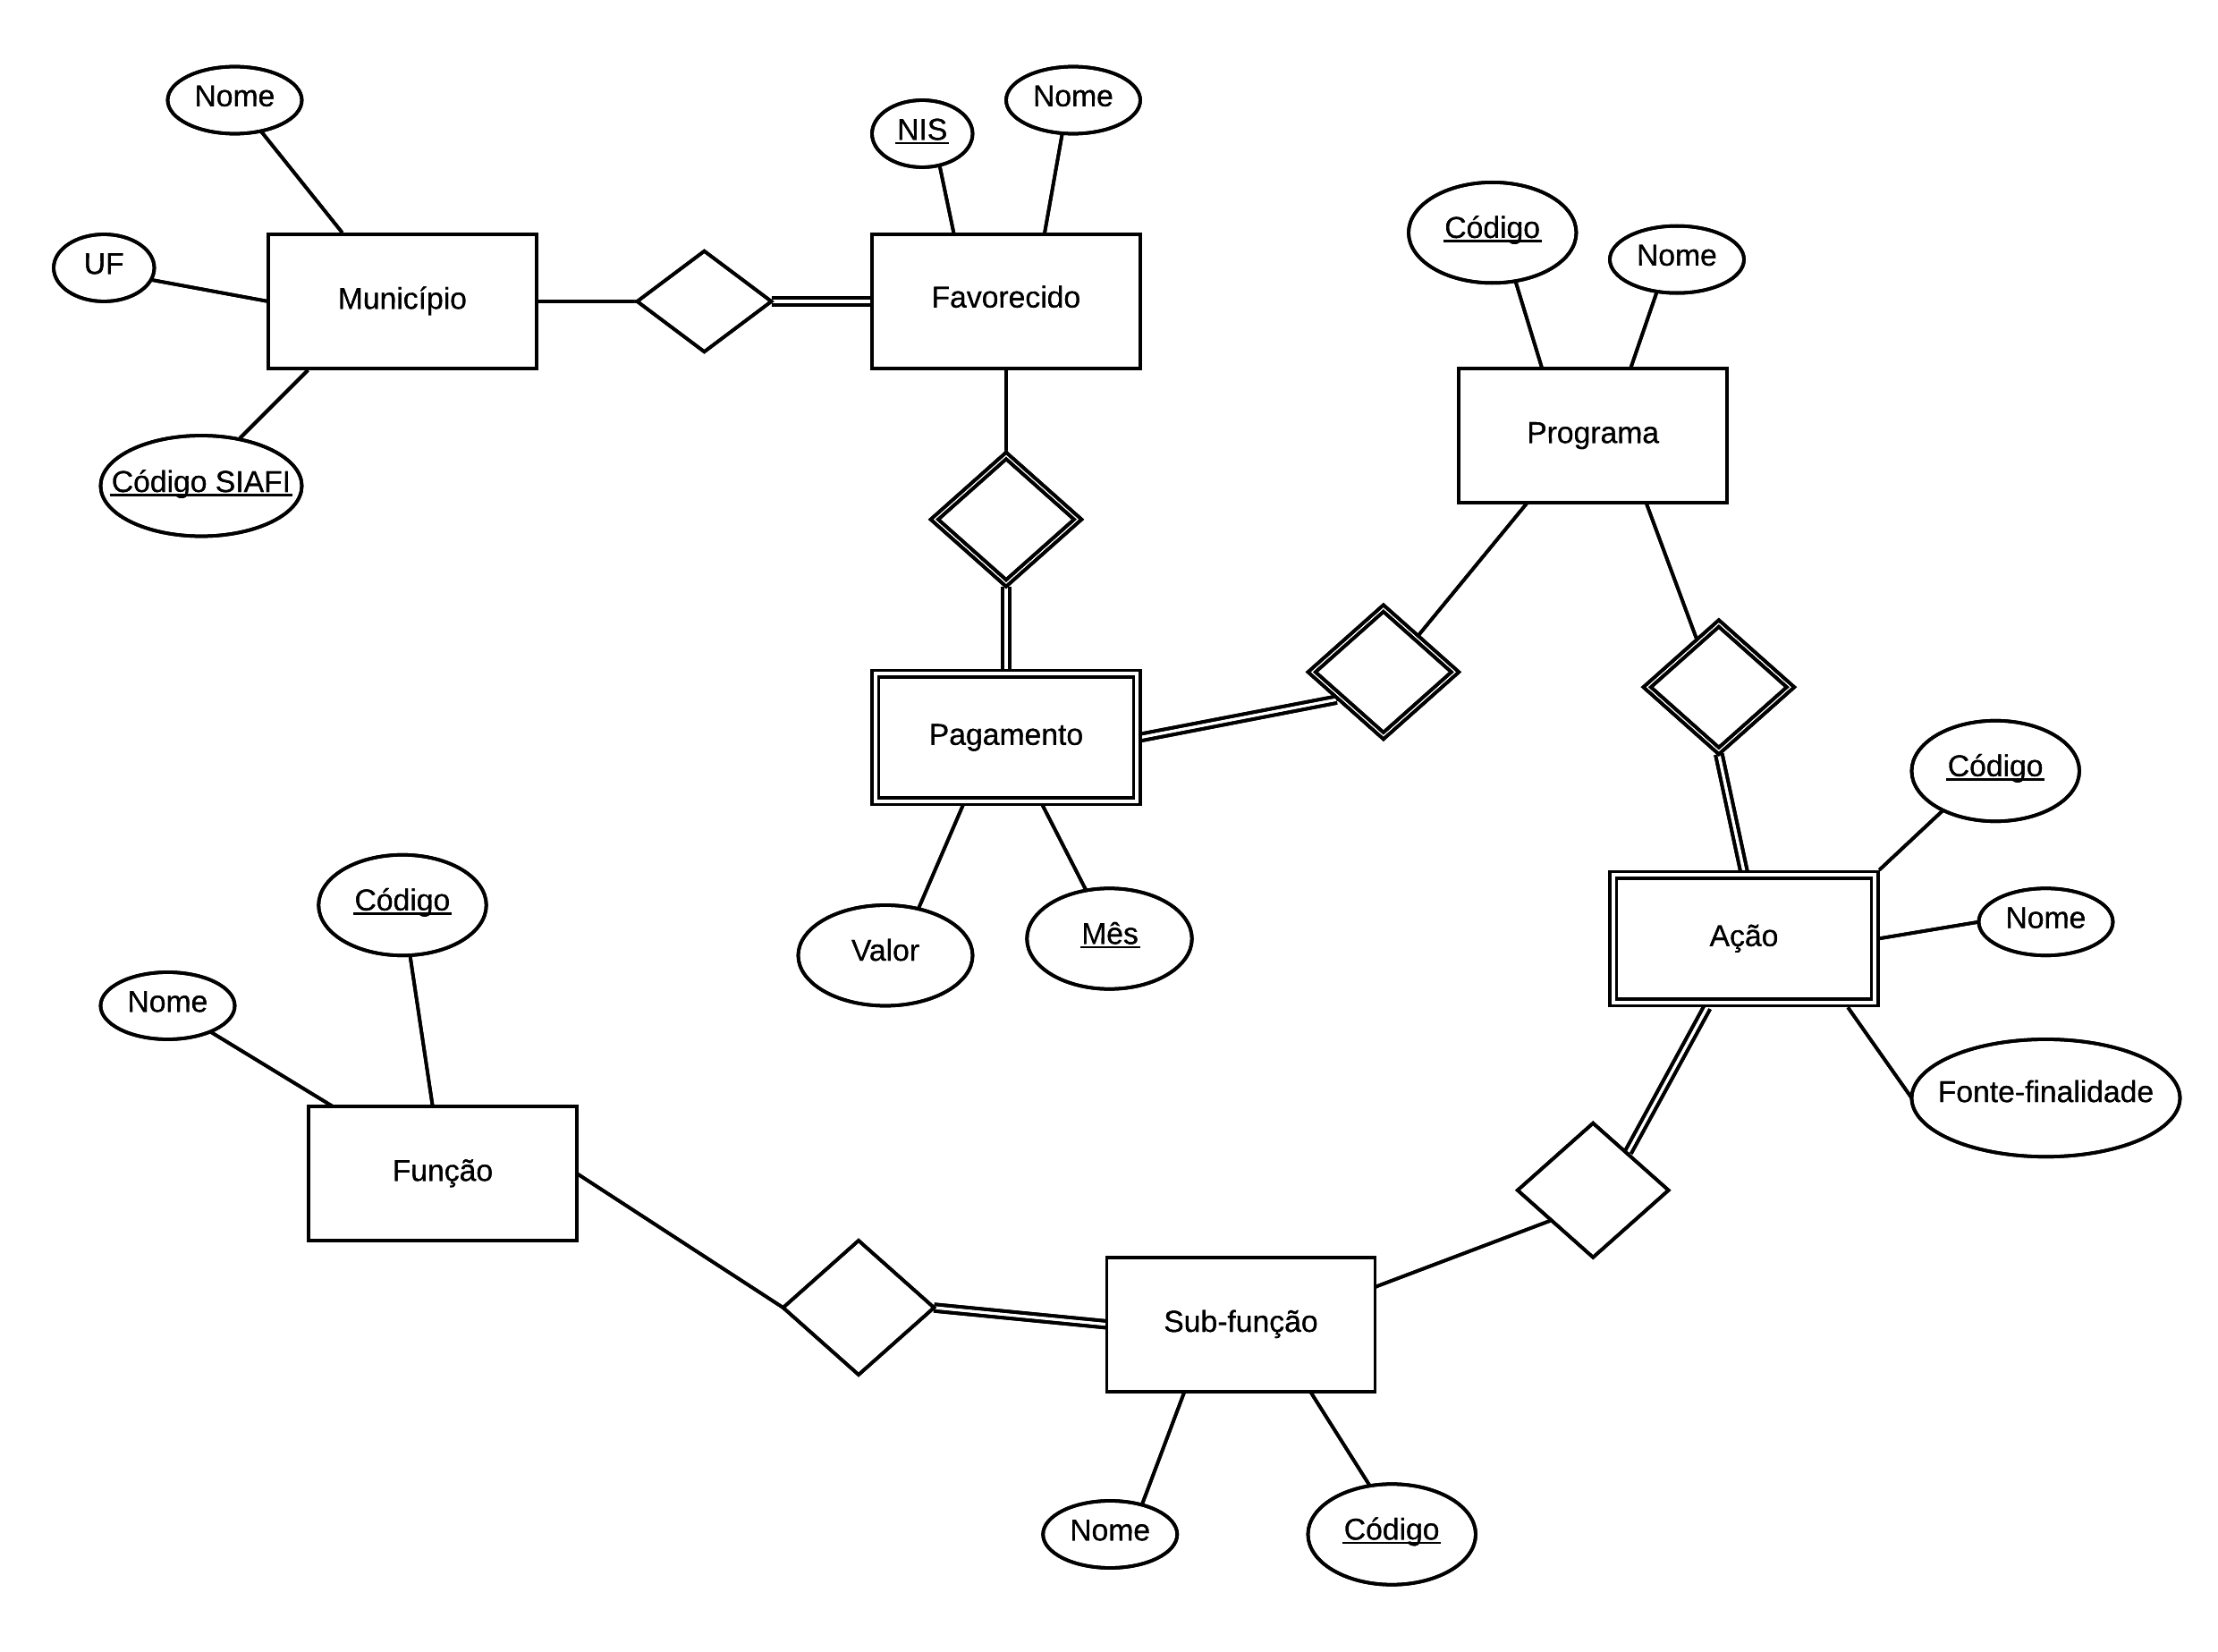
\includegraphics[width=1\textwidth]{der.png}
		\caption{Diagrama de entidade relacionamento do banco de dados dos pagamentos do Programa Bolsa Família (PBF).}
		\label{fig:der}
	\end{figure}
	
	A entidade \textbf{PAGAMENTO} é na verdade uma relação de multiplicidade N:N entre as entidades \textbf{FAVORECIDO} e \textbf{PROGRAMA}, porém, devido o programa utilizado para desenhar o DER, o \cite{lucid} apresentar problemas para inserir as multiplicidades então foi criado outra entidade para representar esta relação.
	
	\subsection{Características dos atributos do DER}
	\label{sec:atr}
	
	\begin{itemize}
		\item \textbf{UF} [MUNICIPIO] \\ Siglas dos estados. Valores repetem na tabela original do Bolsa Família.
		\item \textbf{Nome} [MUNICIPIO] \\ Nome de cada município de origem dos favorecidos, são relacionados ao Código SIAFI do município. Valores repetem na tabela original do Bolsa Família.
		\item \textbf{Código SIAFI} [MUNICIPIO] \\  É o Sistema Integrado de Administração Financeira do Governo Federal que consiste no principal instrumento utilizado para registro, acompanhamento e controle da execução orçamentária, financeira e patrimonial do Governo Federal. Valor é único para cada nome de município distinto. Valores repetem na tabela original do Bolsa Família.
		\item \textbf{Nome} [FAVORECIDO] \\ Nome de cada favorecido que recebeu pagamento do programa do bolsa família no ano de 2015 e mês de Setembro. Às vezes as folhas de pagamento contém retroativos de pagamento para algum favorecido, portanto, os valores de nome dos favorecidos repetem na tabela original do Bolsa Família.
		\item \textbf{NIS} [FAVORECIDO] \\ É uma solução que permite a identificação do trabalhador nos diversos cadastros, bem como do cidadão brasileiro beneficiário de Programas Sociais e/ou que se enquadre nas condições estabelecidas pelas Políticas Públicas de Governo Federal, Estadual ou Municipal. O NIS - Número de Identificação Social é um número de cadastro e devem ser cadastrados: o trabalhador, vinculado à empresa privada, cooperativa ou empregador pessoa física; os beneficiários de Programas Sociais (cadastrados pelo agente definido pelo Gestor do Programa); o diretor não-empregado quando optante pelo FGTS e os beneficiários de Políticas Públicas (cadastrados pela SRTE, MS e MEC). Como foi citado acima as folhas de pagamento contém retroativos de pagamento para algum favorecido, portanto, os valores de NIS dos favorecidos também repetem na tabela original do Bolsa Família.
		\item \textbf{Código} [PROGRAMA] \\  O código do programa bolsa família. Além disso, as famílias que atendem aos critérios do Programa Bolsa Família e estão inscritas em outros programas federais também têm direito ao benefício (\cite{caixa}). Os valores do código de programa podem variar em outras planilhas, porém, como está em estudo somente o programa do bolsa família o valor do código é único.
		\item \textbf{Nome} [PROGRAMA] \\ Nome oficial do programa do bolsa família oferecido pelo Governo Federal.
		\item \textbf{Código} [ACAO] \\ Código da ação do bolsa família. Análogo ao código de programa. 
		\item \textbf{Nome} [ACAO] \\ Nome oficial da ação do bolsa família oferecido pelo Governo Federal.
		\item \textbf{Fonte-Finalidade} [ACAO] \\ Possui valor igual para todos os dados da planilha coletada do portal da transparência.
		\item \textbf{Nome} [SUBFUNCAO] \\ Nome da classificação sub-funcional da despesa, exemplo: Ação Legislativa, Controle externo, etc.
		\item \textbf{Código} [SUBFUNCAO] \\ Código da classificação sub-funcional da despesa.
		\item \textbf{Nome} [FUNCAO] \\ Nome da classificação funcional da despesa, exemplo: Legislativa, Judiciária, etc.
		\item \textbf{Código} [FUNCAO] \\ Código da classificação funcional da despesa.
	\end{itemize}
	
	\subsection{Entidades do DER}
	\label{sec:ent}
	
	\begin{itemize}
		\item \textbf{MUNICIPIO} \\ Temos que a entidade \textbf{MUNICIPIO} possui 3 atributos: Nome, Código SIAFI (PK) e UF. Decidimos colocar UF como atributo pois não haveria utilidade de uma entidade para UF em si. O Código SIAFI foi escolhido como PK pela característica de ser único para cada valor de nome de município como foi descrito na seção anterior. 
		\item \textbf{FAVORECIDO} \\ Tem 2 atributos: Nome e NIS (PK). O NIS foi escolhido como PK pela característica de ser único para cada valor de nome de favorecido como foi descrito na seção anterior. 
		\item \textbf{PAGAMENTO} \\ Consiste de 2 atributos próprios: Valor e Mês, o Mês é uma das chaves PK. A chave também é composta pelo NIS do favorecido relacionado e Código do programa que o favorecido. A decisão da chave ser composta por estes 3 atributos é devido à repetição dos valores de Código do programa e NIS do favorecido por causa dos retroativos da folha, porém, dois favorecidos de um mesmo programa não podem receber dois pagamentos do mesmo mês e ano, portanto, se tornando crucial a composição destes 3 atributos.
		\item \textbf{PROGRAMA} \\ Possui dois atributos: Código (PK) e Nome. O Código do programa foi escolhido como PK pela característica de ser único para cada valor de nome do programa como foi descrito na seção anterior. 
		\item \textbf{ACAO} \\ Possui 3 atributos próprios: Código (PK), Nome e Fonte-finalidade. O código da ação é PK da entidade pois ele é único para cada valor de nome da ação e fonte-finalidade como foi descrito na seção anterior.  
		\item \textbf{SUBFUNCAO} \\ Contém 2 atributos: Nome e Código (PK). O código da subfunção é PK da entidade pois ele é único para cada valor de nome da subfunção como foi descrito na seção anterior.
		\item \textbf{FUNCAO} \\ Contém 2 atributos: Nome e Código (PK). O código da função é PK da entidade pois ele é único para cada valor de nome da função como foi descrito na seção anterior.
	\end{itemize}

	\subsection{Relações do DER}
	\label{sec:rel}
	
	\begin{itemize}
		\item \textbf{MUNICIPIO} R \textbf{FAVORECIDO} - 1:N \\ Relação de participação parcial x Relação de participação total \\ Um município pode conter N favorecidos e 1 favorecido só pode vir de um município. 
		\item \textbf{FAVORECIDO} R \textbf{PAGAMENTO} - 1:N \\ Relação de participação parcial x Relação de participação total e de identificação \\ Um favorecido pode receber N pagamentos e 1 pagamento de determinado mês/ano pode ir somente para um favorecido.
		\item \textbf{PAGAMENTO} R \textbf{PROGRAMA} - N:1 \\ Relação de participação total x Relação de participação parcial \\ Um pagamento é direcionado a um determinado programa do governo e um programa pode emitir N pagamentos para os favorecidos.
		\item \textbf{PROGRAMA} R \textbf{ACAO} - 1:N \\ Relação de participação parcial x Relação de participação total e de identificação \\ Um programa pode conter N ações e uma ação pertence a um programa.
		\item \textbf{ACAO} R \textbf{SUBFUNCAO} - N:1 \\ Relação de participação total x Relação de participação parcial \\ Uma ação advém de uma subfunção e uma subfunção pode realizar N ações.
		\item \textbf{SUBFUNCAO} R \textbf{FUNCAO} - N:1 \\ Relação de participação total x Relação de participação parcial \\ Uma subfunção pertence a uma determinada função geral e uma função possui N subfunções.
	\end{itemize}
	
	\section{Modelo Relacional (MR)} 
	\label{sec:mr}

	\section{Formas Normais}
	\label{sec:fnormais}
	
	\subsection{1F}
	\label{sec:1f}
	
	\subsection{2F}
	\label{sec:2f}
	
	\subsection{3F}
	\label{sec:3f}
	
	\section{Script geral}
	\label{sec:scriptg}
	
	\section{ETL}
	\label{sec:etl}
	
	\section{Camadas}
	\label{sec:camadas}
	
	\subsection{Persistência}
	\label{sec:pers}
	
	\subsection{GUI}
	\label{sec:gui}
	
	\section{Consultas} 
	\label{sec:consultas}
	
	\section{Views}
	\label{sec:views}
	
	\section{Procedure}
	\label{sec:procedure}
	
	\section{Trigger}
	\label{sec:trigger}
	
	\section{Solução das Perguntas}
	\label{sec:analisep}
	
	\section{Análise dos Resultados}
	\label{sec:resultados}
	
	\section{Conclusão}
	\label{sec:conclusao}
	
\bibliographystyle{sbc}
\bibliography{relatorio} 

%\newpage 
	
\end{document}
